\documentclass[11pt]{article}

\usepackage[utf8]{inputenc}
\usepackage{amsmath, amssymb, amsthm, physics}
\usepackage{geometry}
\usepackage{hyperref}
\usepackage{enumitem}
\usepackage{tikz}
\usetikzlibrary{shapes.geometric, arrows.meta, positioning, fit, backgrounds, calc}

\geometry{letterpaper, margin=1in}

\hypersetup{
    colorlinks=true,
    linkcolor=blue,
    citecolor=blue,
    urlcolor=blue
}

\newtheorem{theorem}{Theorem}
\newtheorem{lemma}{Lemma}

\title{Exact Classical Simulation of Quantum Circuits via a Decoupled Clifford Frame and Active Statevector}
\author{}
\date{}

\begin{document}

\maketitle

\begin{abstract}
\noindent The classical simulation of universal fault-tolerant quantum circuits is limited by the exponential scaling of non-Clifford operations. Standard statevector simulators require memory scaling with the total number of physical qubits, while Stabilizer Rank and generalized stabilizer methods scale with the total number of non-Clifford gates, struggling with deep algorithmic logic. We present a hybrid simulation architecture that decouples the deterministic coordinate transformations of a quantum circuit from its probabilistic complex amplitudes. By factoring the quantum state into an offline classical Clifford frame and an online localized statevector, our method scales exponentially only with the peak number of simultaneously active non-Clifford virtual qubits. This enables the compilation of heavy $\mathcal{O}(n^2)$ matrix tracking prior to runtime execution, allowing a minimal-overhead virtual machine to evaluate exact statevector folding and Pauli frame tracking using zero-cost dimensional expansions and division-free array updates.
\end{abstract}

\section{Introduction}

The efficient classical simulation of quantum circuits is a critical tool for verifying quantum algorithms and designing fault-tolerant architectures. By the Gottesman-Knill theorem, circuits composed exclusively of Clifford gates and Pauli measurements can be simulated efficiently in polynomial time. However, achieving universal quantum computation requires the inclusion of non-Clifford gates, such as the $T$ gate or Toffoli gate. The introduction of these operations generally causes the classical simulation cost to scale exponentially.

Standard Schrödinger-style statevector simulators track the complex amplitudes of the entire computational basis, requiring memory that scales as $\mathcal{O}(2^n)$ for an $n$-qubit system. This restricts exact simulations to approximately 40--50 qubits regardless of circuit depth or structure. To circumvent this, alternative approaches leverage the stabilizer formalism. For instance, Stabilizer Rank methods \cite{bravyi2019} represent the state as a linear combination of stabilizer tableaus, yielding a simulation cost that scales exponentially with the total number of non-Clifford gates. While effective for highly sparse circuits, this exponential scaling with $T$-count renders the simulation of deep arithmetic logic intractable. Generalized stabilizer methods \cite{yoder2012, li2025soft} avoid $T$-count scaling but require tracking a sparse statevector across the full $2^n$ basis, accumulating significant $\mathcal{O}(n^2)$ overhead per shot during dynamic execution.

In this work, we propose a simulation architecture that scales exponentially only with the \textit{peak active virtual qubits}. By maintaining a single deterministic Clifford frame and confining non-Clifford interference strictly to a dynamically sized statevector, we isolate the computational overhead to the subset of virtual qubits actively participating in non-Clifford entanglement.

\section{Circuit Composition and the Heisenberg Picture}
\label{sec:heisenberg}

A quantum circuit over $n$ qubits is a discrete sequence of operations. We partition these operations into two sets:
\begin{enumerate}
    \item \textbf{Deterministic Operations:} Clifford unitaries $C \in \mathcal{C}_n$.
    \item \textbf{Active Operations:} Non-Clifford unitaries (e.g., the $T$ gate), projective Pauli measurements, stochastic Pauli noise, and classically controlled Pauli operations.
\end{enumerate}

To simulate the state evolution efficiently, we shift from the Schrödinger picture to a hybrid formulation utilizing the Heisenberg picture. Because the Clifford group $\mathcal{C}_n$ normalizes the Pauli group $\mathcal{P}_n$, any physical Clifford gate applied to the state can be viewed instead as a passive transformation of the coordinate system.

Let $U_C^{(t)}$ be the cumulative Clifford frame representing all deterministic coordinate transformations up to time $t$. For any physical active operation $O$ applied in the laboratory basis at time $t$, its Pauli generator $P_O$ can be mapped backward into the static virtual basis:
\begin{equation} \label{eq:heisenberg_map}
    \tilde{P}_O = (U_C^{(t)})^\dagger P_O U_C^{(t)}
\end{equation}
Because physical active operations in standard gate sets are generated by local Pauli operators (e.g., measuring $Z_q$, applying noise $X_q$, or rotating via $T = \exp(-i \frac{\pi}{8} Z_q)$), the conjugated virtual generator $\tilde{P}_O$ is guaranteed to map to a valid, albeit multi-qubit, virtual Pauli string.

While this mapping is standard for unitary evolution, it remains valid for non-unitary operations. Consider a projective Pauli measurement of an observable $M$, which collapses the state via the projector $\Pi_{\pm} = \frac{1}{2}(I \pm M)$. Because matrix conjugation distributes linearly over addition, conjugating this projector by the Clifford frame yields:
\begin{equation}
    (U_C^{(t)})^\dagger \left[ \frac{1}{2} \Big( I \pm M \Big) \right] U_C^{(t)} = \frac{1}{2} \Big( I \pm (U_C^{(t)})^\dagger M U_C^{(t)} \Big) = \frac{1}{2} \Big( I \pm \tilde{M} \Big) = \tilde{\Pi}_{\pm}
\end{equation}
Furthermore, because $U_C^{(t)}$ is a unitary matrix, the norm of the state is identically preserved: $\| \Pi_{\pm} |\psi^{(t)}\rangle \|^2 = \| \tilde{\Pi}_{\pm} |\psi_{\text{virtual}}\rangle \|^2$. Thus, projecting onto $M$ in the physical laboratory frame and computing its probability is mathematically equivalent to projecting onto the mapped Pauli string $\tilde{M}$ in the virtual frame.

The same linear distribution applies to stochastic Pauli noise channels and classically controlled Pauli operations. This establishes that the coordinate mapping of the entire quantum circuit is defined by Pauli tracking, independent of the complex amplitudes of the quantum state.

\section{The Factored State Representation}
\label{sec:representation}

We leverage this decoupling to define the exact physical quantum state at time $t$ via a factored representation:
\begin{equation} \label{eq:factored_state}
    |\psi^{(t)}\rangle = \gamma^{(t)} U_C^{(t)} P^{(t)} \Big( |\phi^{(t)}\rangle_A \otimes |0\rangle_D \Big)
\end{equation}
The components of this representation are defined as follows:
\begin{itemize}
    \item $U_C^{(t)} \in \mathcal{C}_n$ is the \textbf{Clifford Frame}, stored in classical memory as a standard $n$-qubit stabilizer tableau. It tracks the logical coordinate system mapping virtual qubits to physical qubits.
    \item $P^{(t)} \in \mathcal{P}_n$ is the \textbf{Pauli Frame}. It is defined strictly in the \textit{virtual} basis and tracks discrete bit-flips and phase-flips. To avoid heavy matrix multiplication, the virtual machine tracks $P^{(t)}$ as binary integers via bitwise XOR operations ($\oplus$), explicitly extracting any resulting Pauli group multiplication phases ($\pm 1, \pm i$) into $\gamma^{(t)}$. Tracking $P^{(t)}$ explicitly avoids the computational expense of iterating over the statevector to multiply amplitudes dynamically.
    \item $A$ and $D$ are the disjoint sets of \textbf{Active} and \textbf{Dormant} virtual qubits, respectively, where $|A| = k$ and $|D| = n-k$.
    \item $|\phi^{(t)}\rangle_A \in \mathbb{C}^{2^k}$ is the \textbf{Active Statevector}. It is a dense, unnormalized complex array of size $2^k$ that exclusively tracks non-Clifford superposition.
    \item $\gamma^{(t)} \in \mathbb{C}$ is a \textbf{Global Scalar} tracking the continuous global phase and overall physical norm, facilitating deferred scalar division during measurements.
\end{itemize}

Because $P^{(t)}$ is applied \textit{before} the Clifford frame $U_C^{(t)}$ (reading Equation~\ref{eq:factored_state} from right to left), it acts directly on the abstract virtual qubits. If a physical Pauli error or measurement byproduct $E_{\text{lab}}$ occurs in the laboratory, we map it to the virtual basis via $\tilde{E}_{\text{virtual}} = (U_C^{(t)})^\dagger E_{\text{lab}} U_C^{(t)}$, and update the Pauli frame via a bitwise XOR: $P^{(t)} \leftarrow P^{(t)} \oplus \tilde{E}_{\text{virtual}}$, extracting any resulting phase into $\gamma^{(t)}$.

At $t=0$, the system is initialized in the standard computational all-zero state: $U_C = I$, $P = I$, $D$ contains all $n$ qubits, $A$ is empty ($k=0$), $|\phi\rangle_A = [1]$, and $\gamma = 1$.

\section{Virtual Operations and Coordinate Compression}
\label{sec:virtual_ops}

To apply a mapped virtual operation, standard statevector simulators evaluate multi-qubit Pauli strings directly across their entire memory array. We instead geometrically compress the generators onto a single virtual qubit $v$ prior to array evaluation.

\subsection{Basis Transformations and Pauli Compression}
Suppose a physical operation is generated by a multi-qubit virtual Pauli string $\tilde{P} \propto X^{\mathbf{x}} Z^{\mathbf{z}}$. We apply a sequence of virtual Clifford gates $V \in \mathcal{C}_n$ exclusively to the virtual qubits such that $V \tilde{P} V^\dagger = P_v$, where $P_v \in \{X_v, Z_v\}$. The sequence $V$ is determined constructively by an Ahead-Of-Time (AOT) compiler using an $\mathcal{O}(n)$ algorithm based on a greedy Pauli reduction.

\begin{lemma}[Zero-Cost Dormant Property]
If the virtual transformation $V$ utilizes a controlled gate (CNOT or CZ) where the control is a dormant qubit $q \in D$, the gate acts as the identity on the computational zero state $|0\rangle_D$. Thus, the active statevector $|\phi\rangle_A$ remains invariant.
\end{lemma}

\begin{lemma}[Exact Pauli Compression]
\label{lem:pauli_compression}
For any non-identity $n$-qubit virtual Pauli operator $\tilde{P} \in \mathcal{P}_n$, there exists a sequence of at most $2n$ virtual Clifford gates $V \in \mathcal{C}_n$ such that $V \tilde{P} V^\dagger = \gamma P_v$, where $P_v \in \{X_v, Z_v\}$ acts non-trivially on exactly one virtual qubit $v$, and $\gamma \in \{\pm 1, \pm i\}$.
\end{lemma}

\begin{proof}
Let the multi-qubit operator be parameterized by its Boolean support vectors $\mathbf{x}, \mathbf{z} \in \{0,1\}^n$ such that $\tilde{P} \propto X^{\mathbf{x}} Z^{\mathbf{z}}$. We construct $V$ in two mutually exclusive cases:

\textbf{Case 1 ($\mathbf{x} \neq \emptyset$):} The operator contains $X$-basis support. Select a pivot virtual qubit $v$ such that $x_v = 1$. For every other qubit $q \neq v$ where $x_q = 1$, append $\text{CNOT}_{v \to q}$ to $V$. By the conjugation relations of the Pauli normalizer:
\begin{equation}
    \text{CNOT}_{v \to q} (X_v \otimes X_q) \text{CNOT}_{v \to q}^\dagger = (X_v \otimes I_q)(I_v \otimes X_q) = X_v \otimes I_q
\end{equation}
This deterministically annihilates the $X$-support on $q$. Any $Z$-support on $v$ or $q$ propagates to a new vector $\mathbf{z}'$. Thus, the intermediate operator reduces strictly to $\tilde{P}' \propto X_v \otimes Z^{\mathbf{z}'}$.

Next, to eliminate the remaining $Z$-support, append $\text{CZ}_{v, q}$ to $V$ for every $q \neq v$ where $z'_q = 1$. Because the controlled-Z gate applies a symmetric conditional phase, its conjugation rule yields:
\begin{equation}
    \text{CZ}_{v, q} (X_v \otimes Z_q) \text{CZ}_{v, q}^\dagger = (X_v \otimes Z_q)(I_v \otimes Z_q) = X_v \otimes I_q
\end{equation}
This strictly annihilates the $Z$-support on all $q \neq v$ without altering the $X_v$ pivot. The operator is now fully localized to $v$ as either $X_v$ or $Y_v$. If it is $Y_v$, appending a virtual Phase gate ($S_v$) yields $S_v Y_v S_v^\dagger = -X_v$. The operator is successfully compressed to $X_v$.

\textbf{Case 2 ($\mathbf{x} = \emptyset$):} The operator is a pure $Z$-string ($\mathbf{z} \neq \emptyset$). Select a pivot $v$ such that $z_v = 1$. For every $q \neq v$ where $z_q = 1$, append $\text{CNOT}_{q \to v}$ (control $q$, target $v$) to $V$. Under conjugation:
\begin{equation}
    \text{CNOT}_{q \to v} (Z_q \otimes Z_v) \text{CNOT}_{q \to v}^\dagger = (Z_q \otimes I_v)(Z_q \otimes Z_v) = I_q \otimes Z_v
\end{equation}
This annihilates the $Z$-support on all $q \neq v$. The operator is successfully compressed to $Z_v$.

Because each applied two-qubit gate monotonically erases generator support on qubit $q$ without spreading tensor factors to previously cleared qubits, the sequence $V$ requires at most $\mathcal{O}(n)$ local Clifford gates and mathematically guarantees isolation to a single virtual qubit.
\end{proof}

To maximize zero-cost compression, the compiler implements the constructive procedure from Lemma~\ref{lem:pauli_compression}, applying specific heuristics when selecting the pivot $v$ to preserve the dormant state:
\begin{enumerate}
    \item \textbf{$X$-Compression Pivot Selection:} When selecting the pivot $v \in \mathbf{x}$ to fold the $X$-support, the compiler preferentially chooses $v \in D$. Because the resulting $\text{CNOT}_{v \to q}$ operations use $v$ as the control, selecting a dormant control ensures the geometric fold evaluates at zero runtime cost (by Lemma 1). If the compiler is forced to select a pivot $v \in A$, it is strictly because $\mathbf{x} \cap D = \emptyset$. Consequently, all target qubits $q \in \mathbf{x}$ are guaranteed to also be in $A$, ensuring $X$-compression never inadvertently activates a dormant qubit.
    \item \textbf{$Z$-Compression Pivot Selection:} Following $X$-compression, the $Z$ support is updated to some new set $\mathbf{z}'$.
    \begin{itemize}
        \item \textit{If $\mathbf{x} \neq \emptyset$ (Operator contains $X_v$):} The pivot $v$ is already fixed from $X$-compression, and the necessary $\text{CZ}$ gates are applied as described in Lemma~\ref{lem:pauli_compression} to erase the remaining $Z$-support.
        \item \textit{If $\mathbf{x} = \emptyset$ (Pure $Z$-string):} The compiler selects a new pivot $v \in \mathbf{z}'$, preferentially choosing $v \in A$. Because the required $\text{CNOT}_{q \to v}$ gates use $q$ as the control, preferring $v \in A$ maximizes the chance that the controls $q$ are dormant, executing efficiently without needlessly expanding the active statevector.
    \end{itemize}
\end{enumerate}

If the resulting compressed generator is $Y_v$, the compiler appends a virtual Phase gate ($S_v$) to map it to $X_v$. Because mapped generators evolve by matrix conjugation ($S_v Y_v S_v^\dagger = -X_v$), this mathematically negates the physical operation's generator. For a non-Clifford rotation, the compiler inverts the rotation angle rather than absorbing a scalar phase into $\gamma$.
Mathematically, let $O(\tilde{P})$ represent the physical operation constructed from the mapped generator. We insert the identity $V^\dagger V = I$ into Equation~\ref{eq:factored_state} before evaluating it:
\begin{align}
    O(\tilde{P}) \Big[ P \Big( |\phi\rangle_A \otimes |0\rangle_D \Big) \Big] &= V^\dagger \Big[ V O(\tilde{P}) V^\dagger \Big] \big(V P V^\dagger \big) V \Big( |\phi\rangle_A \otimes |0\rangle_D \Big) \nonumber \\
    &= V^\dagger O(P_v) P' \Big( V \big( |\phi\rangle_A \otimes |0\rangle_D \big) \Big)
\end{align}
The Clifford frame absorbs the inverse transformation ($U_C \leftarrow U_C V^\dagger$), the operation $O(P_v)$ based on the compressed generator is isolated, the runtime Pauli tracking frame is dynamically conjugated ($P \leftarrow V P V^\dagger$), and the active statevector undergoes the coordinate transformation $V$. If $V$ requires operations between active qubits, they manifest as division-free array updates.

\subsection{Non-Clifford Evolution (The $T$ Gate)}
\label{sec:t_gate}

Applying a non-Clifford gate, such as a physical $T_q$ gate, relies on this basis compression. Algebraically, we represent the $T_q$ gate using the asymmetric computational basis convention: $T_q = \text{diag}(1, e^{i\pi/4})$. In the Pauli basis, this is equivalent to $e^{i\pi/8}\exp(-i \frac{\pi}{8} Z_q)$. By the Heisenberg mapping, this physical generator maps to a multi-qubit Pauli string $\tilde{Z}_q$.

We apply the virtual Clifford sequence $V$ to compress this generator onto a single virtual qubit $v$, yielding $P_v$. Because $V$ is a unitary transformation, it distributes algebraically into the exponent's Taylor series expansion:
\begin{equation}
    V \exp\left(-i \frac{\pi}{8} \tilde{Z}_q\right) V^\dagger = \exp\left(-i \frac{\pi}{8} V \tilde{Z}_q V^\dagger\right) = \exp\left(-i \frac{\pi}{8} P_v\right)
\end{equation}
(If compression natively yields $X_v$, appending a virtual $H_v$ ensures the rotation is around $Z_v$).

The Pauli frame $P$ sits in front of the local rotation $\exp(-i \frac{\pi}{8} Z_v)$. Because Pauli matrices commute or anti-commute, commuting the rotation past the Pauli frame algebraically extracts a dynamic sign:
\begin{equation}
    \exp\left(-i \frac{\pi}{8} Z_v\right) P = P \exp\left(-i \frac{\pi}{8} (-1)^c Z_v\right)
\end{equation}
where $c=1$ if $P$ anti-commutes with $Z_v$ (i.e., contains $X_v$ or $Y_v$), and $0$ otherwise. The runtime queries the $X_v$ tracking bit to select whether to apply $T$ or $T^\dagger$.

We evaluate this localized rotation against the virtual statevector in one of three ways:

\textbf{Scalar Phase ($v \in D$, generator natively $Z_v$):} If the compressed generator naturally reduces to $Z_v$ on a dormant qubit, applying the $T$ gate to the $|0\rangle_v$ state acts as the identity (yielding a scalar phase of $1$). However, if the dynamically conjugated Pauli frame $P$ contains an $X_v$ parity bit ($\mathbf{p}_{X,v} = 1$), the physical state is $|1\rangle_v$, logically yielding a scalar phase of $e^{i\pi/4}$. The VM queries the tracking bit to select the correct phase. The array is unchanged, and the scalar is absorbed into $\gamma$. No dimensionality expansion is required, yielding a memory reduction.

\textbf{Dimensionality Expansion ($v \in D$, requires $H_v$):} If the generator originally compressed to $X_v$, the necessary virtual $H_v$ gate rotates the dormant state from $|0\rangle_v$ to $|+\rangle_v$. The qubit transitions to active ($A \leftarrow A \cup \{v\}$). The array dimension increments ($k \leftarrow k+1$) and doubles in size via a tensor product: $|\phi\rangle_A \leftarrow |\phi\rangle_A \otimes \begin{bmatrix} 1 \\ 1 \end{bmatrix}$. The normalization factor of $1/\sqrt{2}$ is absorbed into $\gamma$, and the local $T$ rotation is then applied to the newly activated axis.

\textbf{Local Phase Application ($v \in A$):} If the compressed rotation targets an already active qubit, the array dimension is unchanged. The diagonal $T$ phase is applied locally to the $|1\rangle$ branch along axis $v$ of the dense complex array $|\phi\rangle_A$, dynamically applying $T^\dagger$ instead of $T$ if the $X_v$ parity bit is set in $P$.

While the derivation above focuses on the $T$ gate, this geometric compression extends to arbitrary non-Clifford operations. Any single-qubit rotation $\exp(-i \theta G)$ compresses to a local rotation using the same unitary distribution.

\subsection{Conditional Pauli Operations (Noise + Feed-Forward)}
\label{sec:conditional_paulis}

We can consider both feed-forward and noise as conditional Pauli operations that depend on a classically boolean variable $c \in \{0, 1\}$. For example, a classically controlled $X$ gate applies $X$ if $c=1$ and the identity if $c=0$. A stochastic Pauli error applies a Pauli operator with some probability, which can be represented as a conditional operation where $c$ is a random bit sampled according to the error probability.
\begin{equation}
    |\psi^{(t+1)}\rangle = (E_{\text{lab}})^c |\psi^{(t)}\rangle = (E_{\text{lab}})^c \left[ \gamma^{(t)} U_C^{(t)} P^{(t)} \Big( |\phi^{(t)}\rangle_A \otimes |0\rangle_D \Big) \right]
\end{equation}

By inserting the identity $U_C^{(t)} (U_C^{(t)})^\dagger = I$, the physical operator is conjugated by the deterministic offline Clifford frame. This maps the operation to a multi-qubit virtual Pauli string $\tilde{E} = (U_C^{(t)})^\dagger E_{\text{lab}} U_C^{(t)}$, shifting the conditional operator into the virtual basis:
\begin{equation}
    |\psi^{(t+1)}\rangle = \gamma^{(t)} U_C^{(t)} (\tilde{E})^c P^{(t)} \Big( |\phi^{(t)}\rangle_A \otimes |0\rangle_D \Big)
\end{equation}

Unlike continuous non-Clifford rotations and projective measurements, which interact with the active statevector and therefore require the geometric compression defined in Section~\ref{sec:virtual_ops}, a conditional Pauli is a discrete operator. It does not require localization to a single virtual qubit. Instead, if the classical condition evaluates to true ($c=1$), the multi-qubit virtual string $\tilde{E}$ is algebraically absorbed directly into the dynamic Pauli frame.

Because the $n$-qubit Pauli group $\mathcal{P}_n$ is closed under multiplication, the product $\tilde{E} P^{(t)}$ analytically resolves to a new Pauli frame $P^{(t+1)}$ alongside an algebraic multiplication phase $\alpha \in \{\pm 1, \pm i\}$. The update to the factored state resolves to:
\begin{equation}
    |\psi^{(t+1)}\rangle = \Big( \gamma^{(t)} \cdot \alpha \Big) U_C^{(t)} P^{(t+1)} \Big( |\phi^{(t)}\rangle_A \otimes |0\rangle_D \Big)
\end{equation}
If the condition evaluates to false ($c=0$), the operators act as the identity ($P^{(t+1)} = P^{(t)}$ and $\alpha = 1$).


\section{Projective Measurements and State Collapse}
\label{sec:measurements}

By compressing any mapped physical observable to a single virtual Pauli operator $Z_v$ or $X_v$, projective measurements reduce to four isolated scenarios evaluated against the virtual state and the dynamic Pauli frame $P$. Let $\mathbf{p}_{X,v}$ and $\mathbf{p}_{Z,v}$ denote the virtual $X$ and $Z$ parities tracked by $P$ on qubit $v$.

\textbf{Case 1: Deterministic Filter (Measure $Z_v$ on $D$).}
Because $v \in D$, the abstract state is strictly $|0\rangle_v$. However, the true physical outcome is deterministically dictated by the Pauli frame. The measurement yields $m = \mathbf{p}_{X,v}$. The statevector and virtual registers are untouched.

\textbf{Case 2: Random Pivot (Measure $X_v$ on $D$).}
Measuring $X_v$ on the abstract $|0\rangle_v$ state yields a 50/50 random outcome $m \in \{0, 1\}$. The abstract qubit collapses to $|\pm\rangle_v$. To restore the dormant computational zero state ($|0\rangle_v$), we apply a virtual Hadamard $H_v$, updating the offline frame $U_C \leftarrow U_C H_v$. Because the projective collapse cleanses the qubit's prior Pauli history, the VM mathematically extracts the algebraic phase $(-1)^{\mathbf{p}_{X,v} \cdot m}$ into $\gamma$. The VM then anchors the computational zero state by resetting the tracking bits directly to $\mathbf{p}_{X,v} = m$ and $\mathbf{p}_{Z,v} = 0$. The active statevector $|\phi\rangle_A$ remains invariant.

\textbf{Case 3: Diagonal Shrink (Measure $Z_v$ on $A$).}
The measurement projects the active statevector along the $Z$-axis. The array probability $P_{\text{arr}}(0)$ is calculated. The mapping of classical outcomes to abstract array branches is swapped if $\mathbf{p}_{X,v} = 1$ (i.e., the physical outcome $m$ corresponds to the abstract branch $m \oplus \mathbf{p}_{X,v}$). After sampling the physical outcome $m$, the array is filtered to keep only the proper abstract branch. The prior $Z$-parity acting on the selected abstract branch yields an algebraic phase of $(-1)^{\mathbf{p}_{Z,v} \cdot (m \oplus \mathbf{p}_{X,v})}$, which is extracted into $\gamma$. The array dimension halves ($k \leftarrow k-1$). The VM anchors the new zero state by resetting the tracking bits to $\mathbf{p}_{X,v} = m$ and $\mathbf{p}_{Z,v} = 0$, and demotes $v$ back to $D$.

\textbf{Case 4: Interfering Shrink (Measure $X_v$ on $A$).}
The active statevector is projected onto the $X$-basis ($|\pm\rangle_v$). The true physical probability relies on the array's $X$-basis superposition, swapping the outcome mapping if $\mathbf{p}_{Z,v} = 1$ (as $Z$ anti-commutes with $X$). Upon sampling $m$, the $|0\rangle_v$ and $|1\rangle_v$ branches of the array fold over each other and interfere via unitarily scaled addition or subtraction ($v'_i = (v_i \pm v_{i+2^{k-1}}) / \sqrt{2}$) dictated by $m \oplus \mathbf{p}_{Z,v}$. Pushing the prior $X$-parity through the $X$-basis measurement collapse yields an algebraic phase of $(-1)^{\mathbf{p}_{X,v} \cdot m}$, which is extracted into $\gamma$. The dimension halves ($k \leftarrow k-1$). A virtual $H_v$ is applied to the frame to reset the measurement axis from $X$ to $Z$. The VM anchors the computational zero state by resetting the tracking bits to $\mathbf{p}_{X,v} = m$ and $\mathbf{p}_{Z,v} = 0$, and demotes $v$ to $D$.

\textbf{Deferred Normalization:} Standard projection requires dividing all elements in $|\phi\rangle_A$ by $\sqrt{P_m}$. We instead apply this division to the global scalar $\gamma$. Because the active array elements are explicitly scaled by $1/\sqrt{2}$ during the $X$-basis fold to strictly preserve unitary magnitude and prevent overflow, the deferred normalization identically matches the diagonal measurement case, requiring only a standard scalar division ($\gamma \leftarrow \gamma / \sqrt{P_m}$).

\section{Software Architecture: Clifford Frame Determinism}
\label{sec:architecture}

The decoupled representation in Equation~\ref{eq:factored_state} reveals a key structural property:
\begin{theorem}[Clifford Frame Determinism]
The evolution of the Clifford Frame $U_C$ and the dimensional bounds of the active set $A$ depend exclusively on the sequence of physical operations. They are independent of probabilistic measurement outcomes, stochastic Pauli errors, or the continuous amplitudes of $|\phi\rangle_A$.
\end{theorem}

This theorem allows us to alter the execution architecture of quantum circuit simulation by partitioning it into two stages:

\textbf{1. Ahead-of-Time (AOT) Compiler (Offline):}
The compiler propagates the mapped operators through the circuit, executing all $\mathcal{O}(n^2)$ matrix tracking for $U_C$ and the virtual basis transformations $V$. Because dimensionality expansion is deterministic, it extracts the peak active dimension ($k_{\max}$) encountered during the entire circuit. The compiler strips away the $n$-qubit frames and emits a linear trace of static $\mathcal{O}(1)$ opcodes.

\textbf{2. Virtual Machine (Online):}
The runtime VM allocates exactly $2^{k_{\max}}$ elements statically at startup. It iterates through the pre-compiled opcodes, evaluating the dense complex array $|\phi\rangle_A$ and the lightweight Pauli frame tracking $P$. Because all heavy tableau logic was compiled away offline, the VM functions as a minimal-overhead runtime environment, maximizing cache-locality and avoiding dynamic memory allocations.

\subsection{Computational Complexity}
\label{sec:complexity}

Clifford Frame Determinism separates the computational complexity into two regimes:

\textbf{AOT Compiler Complexity (Offline):} For a circuit with $n$ physical qubits and $G$ total operations, the offline compiler computes the virtual basis transformations $V$. Compressing a Pauli operator requires at most $\mathcal{O}(n^2)$ binary operations per gate. Thus, the total offline compilation time scales efficiently as $\mathcal{O}(G n^2)$.

\textbf{Virtual Machine Complexity (Online):} Updating the Pauli frame requires $\mathcal{O}(1)$ bitwise operations. Evaluating statevector folding and local phase applications requires updating the active array of size $2^k$, which takes $\mathcal{O}(2^k)$ operations where $k \le k_{\max}$. Thus, the online runtime per active operation is bounded by $\mathcal{O}(2^{k_{\max}})$, avoiding the $\mathcal{O}(n^2)$ overhead of online tableau pivoting.

While the exact dependence of $k_{\max}$ on the total $T$-gate count ($m$) depends on algorithmic uncomputation and intermediate measurements, the AOT compiler calculates $k_{\max}$ deterministically \textit{before} the VM ever executes. For algorithmically dense circuits where non-Clifford gates act heavily upon a localized logical register, $k_{\max}$ remains small and bounded ($k_{\max} \ll m$), allowing the VM to process thousands of $T$ gates with a predictable $\mathcal{O}(2^{k_{\max}})$ overhead.

\section{The Compiler-VM Interface: HIR and Opcodes}
\label{sec:hir_and_vm}

To bridge the offline compilation and the online execution environment, the architecture utilizes a two-tier software design separated by a clean instruction set boundary.

\subsection{The Heisenberg Intermediate Representation (HIR)}

During the initial compiler pass, the physical quantum circuit is translated into the Heisenberg Intermediate Representation (HIR). All deterministic Clifford operations are absorbed into $U_C$, and all active operations are mapped backward into the static virtual basis. By representing the entire circuit as a flat sequence of virtual Pauli generators, the HIR natively exposes the underlying algebraic structure of the circuit, allowing robust global optimization prior to statevector evaluation.

The HIR consists of explicit operation nodes defined entirely by their mapped virtual Pauli operators:
\begin{itemize}
    \item \textbf{\texttt{HIR\_ROTATE}:} Virtual Pauli generator $\tilde{P}$, rotation angle $\theta$.
    \item \textbf{\texttt{HIR\_MEASURE}:} Virtual Pauli observable $\tilde{M}$, classical memory address $c_{\text{out}}$.
    \item \textbf{\texttt{HIR\_NOISE}:} Virtual Pauli error $\tilde{E}$, error probability $p_E$.
    \item \textbf{\texttt{HIR\_FEEDBACK}:} Virtual Pauli operation $\tilde{O}$, classical memory address $c_{\text{in}}$.
\end{itemize}

\subsection{Global Optimization via the HIR}
\label{sec:hir_optimization}

Because the Front-End maps all active operations into the static virtual basis, the HIR represents the quantum circuit as a flat sequence of multi-qubit Pauli generators. This decoupling of the coordinate frame from the statevector amplitudes enables the AOT compiler to perform global algebraic optimization strictly via symplectic geometry and scalar arithmetic.

\textbf{$\mathcal{O}(1)$ Commutation and Stochastic Barriers.}

The commutation of any two quantum operations is determined entirely by their Pauli generators. Let two adjacent HIR nodes be defined by virtual Pauli operators $\tilde{P}_A \propto X^{\mathbf{x}_A} Z^{\mathbf{z}_A}$ and $\tilde{P}_B \propto X^{\mathbf{x}_B} Z^{\mathbf{z}_B}$. The operators commute if and only if their symplectic inner product vanishes:
\begin{equation}
    \langle \tilde{P}_A, \tilde{P}_B \rangle_{\text{symp}} = (\mathbf{x}_A \cdot \mathbf{z}_B) \oplus (\mathbf{z}_A \cdot \mathbf{x}_B) \equiv 0 \pmod 2
\end{equation}
Because this condition evaluates in $\mathcal{O}(1)$ bitwise operations, the compiler greedily reorders \texttt{HIR\_ROTATE} nodes to parallelize operations and cancel inverses across long circuit depths.

Within this reordering, \texttt{HIR\_NOISE} and \texttt{HIR\_MEASURE} nodes act as strict stochastic barriers. If the compiler attempts to commute a coherent rotation $\exp(-i\theta\tilde{P})$ past a stochastic Pauli channel $\tilde{E}$ (or an observable $\tilde{M}$), the reordering is permitted only if $[\tilde{P}, \tilde{E}] = 0$. If they anti-commute, commuting the rotation mathematically conjugates the stochastic generator ($\tilde{E} \exp(-i\theta\tilde{P}) = \exp(+i\theta\tilde{P}) \tilde{E}$), conditionally inverting the rotation angle and altering the physical noise model or measurement basis. The compiler blocks these invalid reorderings, guaranteeing that the exact probabilistic semantics of the circuit are preserved.

\textbf{Angle Fusion and Clifford Absorption.}

When the commutation pass places two \texttt{HIR\_ROTATE} nodes adjacent to each other such that they share the exact same virtual Pauli generator ($\tilde{P}_A = \tilde{P}_B = \tilde{P}$), they are algebraically fused. Because non-Clifford operations are defined as continuous unitary rotations, fusion simplifies to scalar angle addition:
\begin{equation}
    \exp(-i \theta_1 \tilde{P}) \exp(-i \theta_2 \tilde{P}) = \exp(-i (\theta_1 + \theta_2) \tilde{P})
\end{equation}
The compiler replaces both nodes with a single \texttt{HIR\_ROTATE} parameterized by $\theta_{\text{fused}} = \theta_1 + \theta_2$. This summation exposes two deterministic reductions:
\begin{enumerate}
    \item \textbf{Exact Cancellation ($\theta_{\text{fused}} \equiv 0 \pmod{2\pi}$):} The combined rotation evaluates to the identity $I$ (e.g., sequential $T$ and $T^\dagger$ gates mapped to the same virtual axis). The compiler deletes the nodes from the HIR entirely.
    \item \textbf{Clifford Absorption ($\theta_{\text{fused}} \equiv k\frac{\pi}{4} \pmod{2\pi}$):} If the fused angle evaluates to an integer multiple of $\pi/4$, the resulting rotation is an element of the Clifford normalizer. For example, fusing two physical $T$ gates ($\theta_1 = \theta_2 = \pi/8$) yields a rotation of $\pi/4$, which is equivalent to a virtual Phase gate ($S$) generated by $\tilde{P}$. Rather than emitting an active non-Clifford operation, the compiler converts the node into a deterministic coordinate transformation, absorbs it directly into the offline Clifford frame $U_C$, and deletes it from the HIR.
\end{enumerate}

By evaluating these fusions purely in the virtual Pauli basis, the compiler mathematically guarantees that any sequence of non-Clifford operations that algebraically resolves to a Clifford operation is absorbed offline. This minimizes the total number of runtime operations and suppresses unnecessary dimensional expansions of the active statevector.

\subsection{The Schrödinger Virtual Machine (VM)}

Once optimized, the compiler computes the basis compression $V$, bounds $k_{\max}$, and emits executable opcodes.

\textbf{The VM State:} At startup, the VM allocates a fixed execution state:
\begin{enumerate}
    \item \textbf{The Active Statevector ($|\phi\rangle_A$):} A dense, contiguous complex array of exactly $2^{k_{\max}}$ elements, initialized to zero with $|\phi\rangle_0 = 1$.
    \item \textbf{The Pauli Frame ($P$):} Two $n$-bit integers tracking the accumulated virtual $X$ and $Z$ parities ($\mathbf{p}_X, \mathbf{p}_Z$).
    \item \textbf{The Global Scalar ($\gamma$):} A single complex scalar tracking the continuous global phase and unnormalized probability weight.
    \item \textbf{The Classical Memory ($\mathcal{M}$):} A Boolean array for sequential measurement outcomes.
\end{enumerate}

\textbf{The VM Opcodes:} The VM executes the localized physics utilizing $\mathcal{O}(1)$ or array-bound instructions:
\begin{itemize}
    \item \textbf{\texttt{OP\_CNOT}:} Control virtual axis $v_c$ and target virtual axis $v_t$. Performs a deterministic, in-place swap of amplitudes in $|\phi\rangle_A$. The VM must dynamically conjugate the Pauli frame $P$ via bitwise XORs ($\mathbf{p}_{X,v_t} \leftarrow \mathbf{p}_{X,v_t} \oplus \mathbf{p}_{X,v_c}$ and $\mathbf{p}_{Z,v_c} \leftarrow \mathbf{p}_{Z,v_c} \oplus \mathbf{p}_{Z,v_t}$) to properly propagate runtime errors.
    \item \textbf{\texttt{OP\_CZ}:} Control virtual axis $v_c$ and target virtual axis $v_t$. Applies a conditional $-1$ phase to the $|11\rangle$ subspace of $|\phi\rangle_A$. The VM must dynamically conjugate the Pauli frame $P$ via bitwise XORs ($\mathbf{p}_{Z,v_t} \leftarrow \mathbf{p}_{Z,v_t} \oplus \mathbf{p}_{X,v_c}$ and $\mathbf{p}_{Z,v_c} \leftarrow \mathbf{p}_{Z,v_c} \oplus \mathbf{p}_{X,v_t}$).
    \item \textbf{\texttt{OP\_PHASE}:} Target active axis $v$, rotation angle $\theta$. Applies a local diagonal phase rotation to the $|1\rangle$ branch along axis $v$. The VM queries the $\mathbf{p}_{X,v}$ bit of the Pauli frame to apply the correct dynamic sign ($\pm \theta$).
    \item \textbf{\texttt{OP\_MEAS\_STATIC}:} Target virtual axis $v$, classical index $c_{\text{out}}$. Evaluates the outcome deterministically against $\mathbf{p}_{X,v}$ and writes to $\mathcal{M}[c_{\text{out}}]$.
    \item \textbf{\texttt{OP\_MEAS\_RANDOM}:} Target virtual axis $v$, classical index $c_{\text{out}}$. Samples a 50/50 outcome $m$. Extracts the algebraic phase $(-1)^{\mathbf{p}_{X,v} \cdot m}$ into $\gamma$. Resets the tracking bits directly to $\mathbf{p}_{X,v} = m$ and $\mathbf{p}_{Z,v} = 0$, anchoring the zero state. Writes $m$ to $\mathcal{M}[c_{\text{out}}]$.
    \item \textbf{\texttt{OP\_MEAS\_DIAGONAL}:} Target active axis $v$, classical index $c_{\text{out}}$. Calculates absolute probability over $|\phi\rangle_A$, swapping the mapped abstract outcome if $\mathbf{p}_{X,v} = 1$. Filters the array, defers division via $\gamma \leftarrow \gamma / \sqrt{P_m}$, extracts the algebraic phase $(-1)^{\mathbf{p}_{Z,v} \cdot (m \oplus \mathbf{p}_{X,v})}$ into $\gamma$, resets tracking bits to $\mathbf{p}_{X,v} = m$ and $\mathbf{p}_{Z,v} = 0$, and writes to $\mathcal{M}[c_{\text{out}}]$.
    \item \textbf{\texttt{OP\_MEAS\_INTERFERE}:} Target active axis $v$, classical index $c_{\text{out}}$. Calculates absolute probability over $|\phi\rangle_A$, swapping the mapped abstract outcome if $\mathbf{p}_{Z,v} = 1$. Folds the array via scaled addition or subtraction. Defers division via $\gamma \leftarrow \gamma / \sqrt{P_m}$, extracts the algebraic phase $(-1)^{\mathbf{p}_{X,v} \cdot m}$ into $\gamma$, resets tracking bits to $\mathbf{p}_{X,v} = m$ and $\mathbf{p}_{Z,v} = 0$, and writes to $\mathcal{M}[c_{\text{out}}]$.
    \item \textbf{\texttt{OP\_APPLY\_PAULI}:} Virtual Pauli error $P_{\text{err}}$, condition trigger $b$. Evaluates $b$. If true, the VM updates the Pauli frame ($P \leftarrow P \oplus P_{\text{err}}$) and extracts any Pauli group multiplication phase into $\gamma$.
\end{itemize}

\section{Comparison with Contemporary Paradigms}
\label{sec:comparison}

\subsection{Versus Stabilizer Rank Methods (Bravyi et al., 2019)}
The Stabilizer Rank formalism \cite{bravyi2019} approaches non-Clifford simulation by representing the state as a linear combination of independent stabilizer tableaus ($|\psi\rangle = \sum c_\alpha |\phi_\alpha\rangle$).
\begin{itemize}
    \item \textbf{Scaling Bottlenecks:} Stabilizer Rank methods branch the state upon encountering non-Clifford operations, scaling exponentially with the \textit{Total $T$-Count} ($\mathcal{O}(2^{\alpha m})$). It thrives on highly sparse circuits (e.g., Hidden Shift) where $T$ gates are widely distributed. The proposed method scales via \textit{Peak Active Qubits} ($k_{\max}$). It handles infinite $T$-depth provided the non-Clifford entanglement remains spatially localized, but fails if $k_{\max}$ exceeds RAM limits.
    \item \textbf{Execution Paradigm:} Stabilizer Rank utilizes Monte Carlo sampling and fast norm estimation over tableau inner-products, yielding statistical approximations. Our proposed architecture utilizes exact, deterministic statevector folding, guaranteeing absolute probabilities without statistical infidelity.
\end{itemize}

\subsection{Versus Generalized Stabilizer Formalism (SOFT, Li et al., 2025)}
The SOFT simulator \cite{li2025soft} utilizes the generalized stabilizer formalism \cite{yoder2012}, maintaining a single stabilizer tableau paired with a sparse coefficient vector $v$ tracked across the full $2^n$ computational basis.
\begin{itemize}
    \item \textbf{Theoretical Equivalence:} SOFT limits exponential blowup by relying on a ``coset bound for diagonal $T$-layers,'' proving the number of non-zero coefficients $|v|$ is bounded by $2^{|Q|-r_Q}$, where $Q$ is the support of the $T$ gates and $r_Q$ is the number of local $Z$-stabilizers. This bound is an implicit recognition of our explicitly tracked Active set $A$. Our $2^k$ dense statevector isolates the exact same computational subspace as SOFT's sparse $2^{|Q|-r_Q}$ representation.
    \item \textbf{Execution Overhead:} SOFT operates as an \textit{online} simulator. For every individual shot, the processor must dynamically calculate sparse index mappings ($\mathcal{O}(|v|n)$) and execute heavy tableau pivoting and conjugation ($\mathcal{O}(n^2)$) in real time.
    \item \textbf{The Proposed Advantage:} By actively compressing operators via virtual basis transformations, we convert the sparse $2^n$ basis problem into a dense, contiguous $2^k$ array problem. Crucially, by leveraging Clifford Frame Determinism, our AOT compiler computes \textit{all} $\mathcal{O}(n^2)$ tableau manipulations offline. The runtime VM executes zero tableau updates per shot, lowering execution latency compared to generalized sparse tracking.
\end{itemize}

\section{Conclusion}

We have introduced a classical simulation architecture that explicitly factors universal quantum circuits into a deterministic coordinate frame and a localized, probabilistic statevector. By proving that basis tracking is mathematically independent of statevector amplitudes, we shift the $\mathcal{O}(n^2)$ overhead of stabilizer simulation to an offline compiler. The resulting runtime executes exactly the required non-Clifford interference over a dense virtual array. This methodology bridges the gap between statevector and stabilizer simulations, providing a high-performance, exact simulation pathway tailored for the deep, algorithmically dense operations required by fault-tolerant quantum computation.

\appendix
\section{Software Architecture: Shattering the Exponential Walls}
\label{sec:architecture_walls}

Every exact classical simulator of quantum circuits eventually collides with an exponential computational boundary. The complexity of simulating a generic universal quantum circuit is governed by three primary variables: the total number of physical qubits ($N$), the total non-Clifford gate count ($t$), and the peak simultaneous non-Clifford entanglement, or active rank ($k_{\max}$).

Standard Schrödinger statevector simulators scale as $\mathcal{O}(2^N)$, imposing a hard memory limit regardless of circuit structure. ZX-calculus and Stabilizer-Rank methods bypass this spatial limit but scale as $\mathcal{O}(2^{\alpha t})$, hitting a timeout wall on deep, algorithmically dense non-Clifford logic.

The Unitary Compiler Collection (UCC) is architected as a multi-level Ahead-Of-Time (AOT) compiler toolchain specifically for the Fault-Tolerant Quantum Computing (FTQC) era. By physically decoupling the deterministic topological coordinate frame from the probabilistic active statevector, UCC's pipeline systematically isolates and neutralizes the $N$ and $t$ walls prior to runtime. This leaves execution bounded strictly by $\mathcal{O}(2^{k_{\max}})$. Because FTQC algorithms continuously ``cool'' entanglement via frequent syndrome measurements, this $k_{\max}$ boundary remains mathematically stable, allowing the runtime Virtual Machine to execute at trillion-shot scales.

% ==========================================
% TIKZ DIAGRAM: THE THREE WALLS PIPELINE
% ==========================================
\begin{figure*}[htbp]
    \centering
    \resizebox{\textwidth}{!}{
    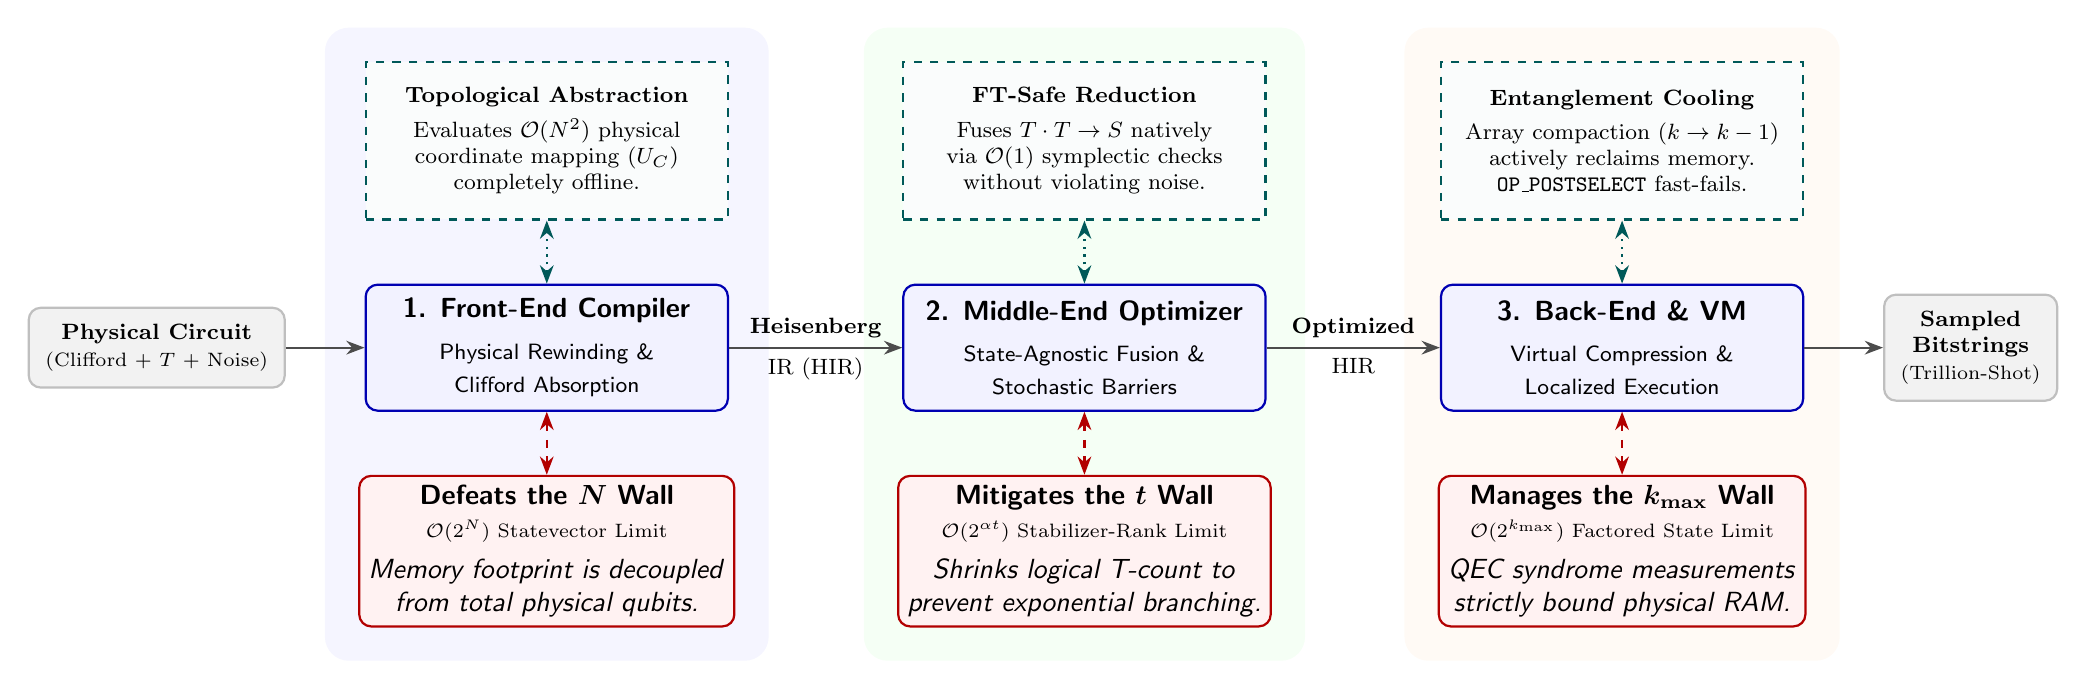
\begin{tikzpicture}[
        >=Stealth,
        font=\sffamily,
        node distance=1.2cm and 2.2cm,
        % Define Styles
        stagebox/.style={rectangle, draw=blue!70!black, fill=blue!5, thick, minimum width=4.6cm, minimum height=1.6cm, align=center, rounded corners=1ex},
        mechbox/.style={rectangle, draw=teal!70!black, fill=teal!2, dashed, thick, minimum width=4.6cm, minimum height=2cm, align=center, font=\footnotesize},
        wallbox/.style={rectangle, draw=red!70!black, fill=red!5, thick, minimum width=4.6cm, minimum height=1.8cm, align=center, rounded corners=1ex},
        data/.style={rectangle, fill=gray!10, draw=gray!50, thick, rounded corners=1ex, font=\footnotesize\bfseries, align=center, inner sep=6pt},
        arrow/.style={->, thick, draw=black!70}
    ]

    % --- STAGE BOXES (Row 2 - The Core Pipeline) ---
    \node[stagebox] (fe) {\textbf{1. Front-End Compiler}\\[1mm] \footnotesize Physical Rewinding \& \\ \footnotesize Clifford Absorption};

    \node[stagebox, right=of fe] (me) {\textbf{2. Middle-End Optimizer}\\[1mm] \footnotesize State-Agnostic Fusion \& \\ \footnotesize Stochastic Barriers};

    \node[stagebox, right=of me] (vm) {\textbf{3. Back-End \& VM}\\[1mm] \footnotesize Virtual Compression \& \\ \footnotesize Localized Execution};

    % --- DATA FLOW (Arrows between stages) ---
    \draw[arrow] (fe) -- node[above, font=\footnotesize\bfseries] {Heisenberg} node[below, font=\footnotesize] {IR (HIR)} (me);
    \draw[arrow] (me) -- node[above, font=\footnotesize\bfseries] {Optimized} node[below, font=\footnotesize] {HIR} (vm);

    % Inputs and Outputs
    \node[data, left=1cm of fe] (input) {Physical Circuit\\ \normalfont\scriptsize (Clifford + $T$ + Noise)};
    \draw[arrow] (input) -- (fe);

    \node[data, right=1cm of vm] (output) {Sampled\\Bitstrings\\ \normalfont\scriptsize (Trillion-Shot)};
    \draw[arrow] (vm) -- (output);

    % --- MECHANISMS (Row 1 - Above Stages) ---
    \node[mechbox, above=0.8cm of fe] (mech1) {\textbf{Topological Abstraction}\\[1mm] Evaluates $\mathcal{O}(N^2)$ physical \\ coordinate mapping ($U_C$) \\ completely offline.};

    \node[mechbox, above=0.8cm of me] (mech2) {\textbf{FT-Safe Reduction}\\[1mm] Fuses $T \cdot T \to S$ natively \\ via $\mathcal{O}(1)$ symplectic checks \\ without violating noise.};

    \node[mechbox, above=0.8cm of vm] (mech3) {\textbf{Entanglement Cooling}\\[1mm] Array compaction ($k \to k-1$) \\ actively reclaims memory. \\ \texttt{OP\_POSTSELECT} fast-fails.};

    \draw[<->, thick, draw=teal!70!black, dotted] (fe) -- (mech1);
    \draw[<->, thick, draw=teal!70!black, dotted] (me) -- (mech2);
    \draw[<->, thick, draw=teal!70!black, dotted] (vm) -- (mech3);

    % --- WALLS DEFEATED (Row 3 - Below Stages) ---
    \node[wallbox, below=0.8cm of fe] (wallN) {\textbf{Defeats the $\boldsymbol{N}$ Wall}\\ \normalfont\scriptsize $\mathcal{O}(2^N)$ Statevector Limit\\[1mm] \textit{Memory footprint is decoupled} \\ \textit{from total physical qubits.}};

    \node[wallbox, below=0.8cm of me] (wallT) {\textbf{Mitigates the $\boldsymbol{t}$ Wall}\\ \normalfont\scriptsize $\mathcal{O}(2^{\alpha t})$ Stabilizer-Rank Limit\\[1mm] \textit{Shrinks logical T-count to} \\ \textit{prevent exponential branching.}};

    \node[wallbox, below=0.8cm of vm] (wallK) {\textbf{Manages the $\boldsymbol{k_{\max}}$ Wall}\\ \normalfont\scriptsize $\mathcal{O}(2^{k_{\max}})$ Factored State Limit\\[1mm] \textit{QEC syndrome measurements} \\ \textit{strictly bound physical RAM.}};

    \draw[<->, thick, draw=red!70!black, dashed] (fe) -- (wallN);
    \draw[<->, thick, draw=red!70!black, dashed] (me) -- (wallT);
    \draw[<->, thick, draw=red!70!black, dashed] (vm) -- (wallK);

    % --- BACKGROUND HIGHLIGHTS (Subtle column grouping) ---
    \begin{scope}[on background layer]
        \node[fill=blue!4, rounded corners=2ex, fit=(mech1)(wallN), inner sep=12pt] {};
        \node[fill=green!4, rounded corners=2ex, fit=(mech2)(wallT), inner sep=12pt] {};
        \node[fill=orange!4, rounded corners=2ex, fit=(mech3)(wallK), inner sep=12pt] {};
    \end{scope}

    \end{tikzpicture}
    }
    \caption{\textbf{The UCC Compilation Architecture.} By factoring the state into a deterministic topological frame and a probabilistic active array, the compiler pipeline systematically targets the three dominant exponential scaling walls of exact quantum simulation ($N$, $t$, and $k$).}
    \label{fig:three_walls_pipeline}
\end{figure*}
% ==========================================

The pipeline functions via three distinct operational layers (Figure~\ref{fig:three_walls_pipeline}):

\subsection{Stage 1: Bypassing the $N$ Wall (State-Agnostic Ingestion)}
Traditional statevector simulators allocate memory as a direct function of $N$, crashing on highly sparse topologies like surface codes at merely $N \approx 40$ physical qubits. The UCC Front-End bypasses this spatial limit by shifting topological tracking entirely offline. By mathematically absorbing all deterministic physical Clifford routing into a classical tableau, empty computational space is never instantiated in memory. Non-Clifford operations and measurements are rewound to the $t=0$ vacuum, producing the Heisenberg Intermediate Representation (HIR)---a purely state-agnostic phase polynomial. Because physical topology is stripped away prior to execution, the Virtual Machine's memory footprint is completely decoupled from the lattice size.

\subsection{Stage 2: Mitigating the $t$ Wall (FT-Safe Optimization)}
Stabilizer-rank algorithms branch exponentially on non-Clifford gates, frequently timing out on algorithmically dense logical operations. The UCC Middle-End mitigates this by functioning as a true AOT compiler to physically shrink the runtime footprint. It sweeps the HIR, utilizing $\mathcal{O}(1)$ symplectic inner products to group operations and statically fuse redundant gates (e.g., $T \cdot T \to S$) prior to execution.

Crucially, the optimizer is strictly \textit{Correct-by-Construction}. Traditional logical optimizers (such as ZX-calculus rewrites) often destroy physical error models by blindly commuting non-Clifford gates past stochastic channels. The UCC optimizer treats \texttt{MEASURE} and \texttt{NOISE} nodes as rigid algebraic barriers, mathematically guaranteeing that hardware noise models are never accidentally conjugated into unphysical bases during $T$-count reduction.

\subsection{Stage 3: Managing the $k_{\max}$ Wall (Entanglement Cooling)}
UCC's execution speed is ultimately bounded by $\mathcal{O}(2^{k_{\max}})$, tracking only the active non-Clifford superposition. For arbitrary random circuits, this dimension grows uncontrollably. However, FTQC algorithms do not allow entanglement to grow unbounded; they actively ``cool'' the state's non-Clifford entropy via continuous syndrome extraction.

The Compiler Back-End and Virtual Machine are natively engineered to exploit this physics. Whenever an active virtual qubit is measured, the Back-End emits specific routing instructions that trigger a division-free \textit{contiguous array compaction}, physically halving the memory size ($k \to k-1$) and averting the fragmented pointer-chasing characteristic of sparse stabilizer methods. Furthermore, to survive trillion-shot evaluations of noisy magic state cultivation, the compiler emits fast-fail \texttt{OP\_POSTSELECT} instructions, allowing the VM to instantly abort doomed logical trajectories the moment a parity check fails, saving deep non-Clifford floating-point operations.

\subsection{Discussion: Continuous Universality}
While this work focuses on optimizing discrete FTQC logic to demonstrate flat memory scaling under syndrome cooling, the underlying Factored State architecture is natively continuous. Unlike Stabilizer Rank or graph-theoretic methods---which are fundamentally restricted to discrete algebraic decompositions---UCC's 32-byte RISC payload accommodates inline continuous complex weights. Future work will leverage the AOT compiler's Dominant Term Factoring to boundedly simulate coherent, continuous circuit-level crosstalk without abandoning the rigorous exactness of the Factored State framework.

\begin{thebibliography}{9}

\bibitem{bravyi2019}
S. Bravyi, D. Browne, P. Calpin, E. Campbell, D. Gosset, and M. Howard,
``Simulation of quantum circuits by low-rank stabilizer decompositions,''
\textit{Quantum}, vol. 3, p. 181, 2019.

\bibitem{li2025soft}
R. Li, K. Zheng, Y. Zhang, H. Lou, S. Ying, K. Liu, and X. Sun,
``SOFT: a high-performance simulator for universal fault-tolerant quantum circuits,''
\textit{arXiv preprint arXiv:2512.23037}, 2025.

\bibitem{yoder2012}
T. J. Yoder,
``A generalization of the stabilizer formalism for simulating arbitrary quantum circuits,''
2012. [Online]. Available: http://www.scottaaronson.com/showcase2/report/ted-yoder.pdf

\end{thebibliography}

\end{document}
